\chapter{Probability in Practice: Implementing Distributions}

The immediate problem with the abstract definitions introduced above
is that they do not provide an explicit means of computing expectations 
in practical applications.  When the sample space is structured, however, 
that structure can be leveraged to provide the explicit implementations we 
need to apply probability theory in practice.  This is particularly evident 
when the sample space is discrete or a subset of the real numbers.

\section{Implementations of Probability Distributions over
Discrete Sample Spaces}

When the sample space is discrete we can completely specify a
probability distribution by assigning probability to only a small
and manageable set of events.  Two particularly convenient sets,
point events and interval events, allow us to implement probability
distributions with probability mass functions and cumulative 
distribution functions, respectively.  

\subsection{Probability Mass Functions}

\emph{Probability mass functions} assign probably to point events,
those events that are lone elements of the original sample space.  
Hence a probability mass function is a just function that assigns a 
probability to each element of the sample space,
%
\begin{equation*}
p : \Theta \rightarrow \left[0, 1\right].
\end{equation*}

In this case more general event probabilities are given by simply summing 
the probability of each element in event,
%
\begin{equation*}
\PP \! \left[ E \right]
=
\sum_{\theta \in E} p \! \left( \theta \right).
\end{equation*}
%
Similarly, expectations are given by summing the probability of each 
element of the sample space, weighted by the function value,
%
\begin{equation*}
\mathbb{E} \! \left[ f \right]
=
\sum_{\theta \in \Theta} f \! \left( \theta \right) p \! \left( \theta \right),
\end{equation*}
%
for any $f \in \mathcal{F} \! \left( \Theta \right)$.

Probability mass functions also have the convenient property that
they are invariant to the particular choice of sample space.  Given
a measurable map $s : \Theta \rightarrow \Omega$ and a probability 
mass function on $\Theta$, we can define an equivalent probability 
mass function on $\Omega$ as
%
\begin{equation*}
p_{\Omega} \! \left( \omega \right) 
\equiv 
p_{\Theta} \! \left( s^{-1} \! \left( \omega \right) \right).
\end{equation*}

\subsection{Conditional Probability Mass Functions}

Probability mass functions can be extended to implement conditional probability
distributions by simply adding a conditioning variable,
%
\begin{equation*}
p_{\Theta \mid \Phi} : \Theta \times \Phi \rightarrow \left[0, 1\right],
\end{equation*}
%
with conditional probabilities and conditional expectations computed
as above,
%
\begin{align*}
\PP_{\Theta \mid \Phi}  \! \left[ E \mid \phi \right]
&=
\sum_{\theta \in E} p_{\Theta \mid \Phi}  \! \left( \theta \mid \phi \right),
\\
\mathbb{E}_{\PP_{\Theta \mid \Phi} } \! \left[ f \mid \phi \right]
&=
\sum_{\theta \in \Theta} f \! \left( \theta \right) 
p_{\Theta \mid \Phi}  \! \left( \theta \mid \phi \right),
\end{align*}

A huge advantage of this representation is that it drastically simplifies the
construction of joint and marginal probability distributions.  Instead of implicitly
defining an abstract joint distribution, for example, we can construct an 
explicit joint probability mass function,
%
\begin{equation*}
p_{\Theta \times \Phi} \! \left( \theta, \phi \right) = 
p_{\Theta \mid \Phi} \! \left( \theta | \phi \right) p_{\Phi} \! \left( \phi \right),
\end{equation*}
%
which readily gives joint probabilities and joint expectations.

Marginalization proceeds similarly -- the marginal probability mass function
is given by simply summing the joint probability mass function over the
nuisance components,
%
\begin{align*}
p_{\Theta} \! \left( \theta \right)
&= 
\sum_{\phi \in \Phi}  p_{\Theta \times \Phi} \! \left( \theta, \phi \right) \\
&=
\sum_{\phi \in \Phi}
p_{\Theta \mid \Phi} \! \left( \theta | \phi \right) p_{\Phi} \! \left( \phi \right).
\end{align*}

\subsection{Cumulative Distribution Functions}

When the sample space is not only discrete but also ordered then we
can also completely specify a probability distribution by assigning
probabilities to \emph{intervals}, 
$\mathcal{I} \! \left( \Theta \right) \subset \mathcal{E} \! \left( \Theta \right)$.
Intervals are events spanning all points less than or equal to some 
distinguished point, $\theta$,
%
\begin{equation*}
I \! \left( \theta \right) = \left\{ \theta' \in \Theta \mid \theta' \leq \theta \right\}.
\end{equation*}
%
The function that assigns these probabilities,
%
\begin{align*}
P 
&: \Theta \rightarrow \mathcal{I} \! 
\left( \Theta \right) \rightarrow \left[0, 1 \right]
\\
&\quad \theta \mapsto 
I \! \left( \theta \right) \;\; \mapsto 
\PP \! \left[ I \! \left( \theta \right) \right].
\end{align*}
%
is called the \emph{cumulative distribution function}.  

As with the probability mass function, cumulative distributions functions
immediately map between sample spaces.  For a measureable map
$s : \Theta \rightarrow \Omega$ we have
%
\begin{equation*}
P_{\Omega} \! \left( I_{\omega} \right) 
\equiv 
P_{\Theta} \! \left( s^{-1} \! \left( I_{\omega} \right) \right).
\end{equation*}

\subsection{Relating Probability Mass Functions and Cumulative 
Distribution Functions}

Because probability mass functions and cumulative distribution functions both
specify the same probability distribution, one can always be used to construct
the other.  Given a probability mass function, for example, we can construct
the cumulative distribution function as
%
\begin{equation*}
P \! \left( \theta \right)
= \PP \! \left[ I \! \left( \theta \right) \right]
= \sum_{\theta' \in I ( \theta )} p \! \left( \theta' \right).
\end{equation*}
%
Similarly, we can construct a probability mass function from a cumulative
distribution function as
%
\begin{equation*}
p \! \left( \theta \right) = 
P \! \left( \theta \right)
- P \! \left( \theta_{-} \right),
\end{equation*}
%
where $\theta_{-}$ is the largest element of $\Theta$ less that $\theta$,
%
\begin{equation*}
\theta_{-} = \max \left\{ \theta' \in \Theta \mid \theta' < \theta \right\}.
\end{equation*}

\section{Implementations of Probability Distributions over the Real
Numbers}

When the sample space is the $D$-dimensional real numbers, or
a subset thereof, there is an uncountably infinite number of point events.  
Not only can we no longer assign a non-zero probability to each point 
event without having most event probabilities explode,
%
\begin{equation*}
\PP \! \left[ E \right] \rightarrow \infty,
\end{equation*}
%
we can't even define the sums over the sample space necessary to 
compute probabilities and expectations!  

Instead of assigning to each point a probability we have to assign  
to each point event a \emph{probability density}  which we can 
\emph{integrate} to give probabilities and expectations.  

Assigning probabilities to intervals, however, is still sufficient so we 
can also define cumulative distribution functions on these spaces.

\subsection{Probability Density Functions}

A \emph{probability density function} assigns a positive value to each
point in the sample space
%
\begin{equation*}
p : \Theta \rightarrow \mathbb{R}^{+}.
\end{equation*}
%
These values, known as \emph{probability densities}, have no particular 
meaning of their own and instead exist only to be integrated to give 
probabilities,
%
\begin{equation*}
\PP \! \left[ E \right]
=
\int_{E} p \! \left( \theta \right) \dd \theta,
\end{equation*}
%
and expectations,
%
\begin{equation*}
\mathbb{E} \! \left[ f \right]
=
\int_{\Theta} f \! \left( \theta \right) p \! \left( \theta \right) \dd \theta.
\end{equation*}

This is an important point that is worth repeating -- probability densities 
are meaningless until they have been integrated over some event.  To 
analogize with physics, the event over which we integrate corresponds 
to a \emph{volume} and the probability given by integrating the density 
over such a volume corresponds to a \emph{mass}.  When we want to 
be careful to differentiate between probabilities and probability densities 
we'll use \emph{probability mass} to refer to the former.

The most awkward properties of probability density functions is that, 
unlike probability mass functions, they do not trivially transform between 
sample spaces.  Specifically, for the measurable map 
$s : \Theta \rightarrow \Omega$
%
\begin{equation*}
p_{\Omega} \! \left( \omega \right)
\neq
p_{\Theta} \! \left( s^{-1} \! \left( \omega \right) \right)!
\end{equation*}

The problem with the real numbers is that mapping between sample
spaces transforms not only the event space but also how we differentiate
and integrate.  Under a well-behaved map $s : \Theta \rightarrow \Omega$ 
the corresponding differential volumes are related by
%
\begin{equation*}
\dd \omega = \left| \mathbf{J} \right| \dd \theta,
\end{equation*}
%
where the matrix
%
\begin{equation*}
J_{ij} 
= 
\frac{\partial \omega_{i} }{ \partial \theta_{j} }
\equiv 
\frac{ \partial s_{i} }{ \partial \theta_{j} }
\end{equation*} 
%
is called the \emph{Jacobian} of the transformation.  Consequently
all integrals are invariant to the particular sample space if and only
if the probability density functions are related by
%
\begin{equation*}
p_{\Omega} \! \left( \omega \right) 
= 
p_{\Theta} \! \left( s^{-1} \! \left( \omega \right) \right) | \mathbf{J} |^{-1}.
\end{equation*}
%
Each sample space has its own differential volume and probability density 
function but \emph{the same integrals} and, hence, the same probabilities 
and expectations (Figure \ref{fig:pdf_transform}).  This dependence on the
sample space is another reason to be careful not to take a probability
density function in isolation too seriously.

\begin{figure*}
\centering
%
\subfigure[]{
%\begin{tikzpicture}[scale=0.3, thick, show background rectangle]
\begin{tikzpicture}[scale=0.3, thick]
  \node[] at (0,0) {
\includegraphics[width=5cm]{density.eps}};
  \foreach \i in {-10.5, -10, ..., 10.5} {
    \draw[-, color=gray80] (-11, \i) to (11, \i);
    \draw[-, color=gray80] (\i, -11) to (\i, 11);
  }  
  \node[] at (0,0) {
\includegraphics[width=5cm]{area.eps}};
  \node[] at (0, -13) { $\PP \! \left[ E_{\Theta} \right] = \int_{E_{\Theta}} 
                                   p_{\Theta} (\theta_{1}, \theta_{2}) 
                                   \dd \theta_{1} \dd \theta_{2} $ };
\end{tikzpicture}
}
%
\subfigure[]{
%\begin{tikzpicture}[scale=0.3, thick, show background rectangle]
\begin{tikzpicture}[scale=0.3, thick]
  \node[] at (0,0) {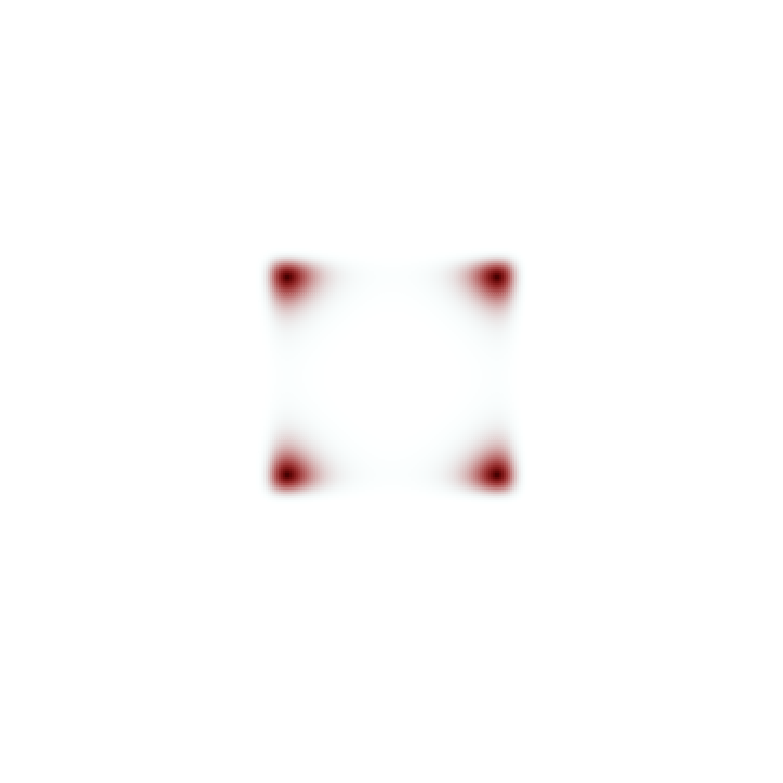
\includegraphics[width=5cm]{transformed_density.eps}};
  \foreach \i in {-10.9969, -10.9428, -10.8857, -10.8251, -10.7605, -10.6915, -10.6174, 
                        -10.5374, -10.4504, -10.355, -10.2497, -10.1319, -9.99835, -9.84419, 
                        -9.66186, -9.4387, -9.15099, -8.74547, -8.05217, 0., 8.05217, 
                        8.74547, 9.15099, 9.4387, 9.66186, 9.84419, 9.99835, 10.1319, 
                        10.2497, 10.355, 10.4504, 10.5374, 10.6174, 10.6915, 10.7605,
                        10.8251, 10.8857, 10.9428, 10.9969} {
    \draw[-, color=gray80] (-11, \i) to (11, \i);
    \draw[-, color=gray80] (\i, -11) to (\i, 11);
  }  
  \node[] at (0,0) {
\includegraphics[width=5cm]{transformed_area.eps}};
  \node[] at (0, -13) { $\PP \! \left[ s \! \left( E_{\Theta} \right) \right] 
                                   = \int_{s(E_{\Theta})} 
                                   p_{\Omega} (\omega_{1}, \omega_{2}) 
                                   \dd \omega_{1} \dd \omega_{2}$ };
\end{tikzpicture}
}
\caption{When sample spaces are real, each sample space has
its own density functions (red), events (green), and differential volumes 
(grey).  Here the sample space in (b) is related to the sample space in 
(a) by the compatible mapping $\left(\omega_{1}, \omega_{2} \right) 
= s \!\left( \theta_{1}, \theta_{2} \right)$. All of these differences, however, 
exactly compensate to ensure that integrals always yield the same 
values, here $\PP \! \left[ E_{\Theta} \right]  = 
\PP \! \left[ s \! \left( E_{\Theta} \right) \right] $.
}
\label{fig:pdf_transform}
\end{figure*}

A helpful mnemonic for the arrangement of the Jacobian in these 
transformations is to remember that the integrand must be invariant,
%
\begin{align*}
p_{\Omega} \! \left( \omega \right) \dd \omega
&=
p_{\Theta} \! \left( \theta \right) \dd \theta
\\
p_{\Omega} \! \left( \theta \right)
&= 
p_{\Theta} \! \left( \theta \right) \frac{ \dd \theta }{ \dd \omega }
\\
p_{\Omega} \! \left( \omega \right)
&= 
p_{\Theta} \! \left( \theta \right) \left| \mathbf{J} \right|^{-1}.
\end{align*}

For a concrete example, consider a two-dimensional sample space 
with real components $\left( \theta_{1}, \theta_{2} \right)$ and a 
probability distribution represented with a Gaussian probability density,
%
\begin{equation*}
p_{\Theta} \! \left( \theta_{1}, \theta_{2} \right)
\propto
\exp \! \left( - \frac{\theta_{1}^{2} + \theta_{2}^{2}}{2} \right).
\end{equation*}
%
We can then introduce a second sample space with the map
%
\begin{equation*}
\left( \omega_{1}, \omega_{2} \right) 
= 
r \! \left( \theta_{1}, \theta_{2} \right) 
= 
\left( s \! \left( \theta_{1} \right), s \! \left( \theta_{2} \right) \right),
\end{equation*}
%
where the component maps are given by
%
\begin{equation*}
s \! \left( \theta \right)
=
\log \! \left(
\frac{ \pi + 2 \, \mathrm{atan} \! \left( \alpha \, \theta \right) }
{ \pi - 2 \, \mathrm{atan} \! \left( \alpha \, \theta \right) }
\right)
\end{equation*}
%
with the inverse
%
\begin{equation*}
s^{-1} \! \left( \omega \right)
=
\frac{1}{\alpha} 
\tan \! \left(
\frac{\pi}{2} \, \frac{e^{\omega} - 1}{e^{\omega} + 1} \right)
\end{equation*}
%
and Jacobian
%
\begin{equation*}
J \! \left( \omega \right)
=
\frac{ \partial s }{ \partial \theta } \! \left( \omega \right)
=
\frac{\alpha}{\pi} \frac{ \left( 1 + e^{\omega} \right)^{2} }{ e^{\omega} }
\sin^{2} \! \left( \frac{ \pi }{ 1 + e^{\omega} } \right).
\end{equation*}
%
The Jacobian of the complete map is then given by
%
\begin{equation*}
\mathbf{J} = 
\begin{bmatrix}
J & 0 \\
0 & J
\end{bmatrix},
\end{equation*}
%
with the determinant $| \mathbf{J} | = J^{2}$.  Hence the transformed
probability density function and differential volume are given by
%
\begin{equation*}
p_{\Omega} \! \left( \omega_{1}, \omega_{2} \right)
=
p_{\Theta} \! \left( 
s^{-1} \! \left( \omega_{1} \right), 
s^{-1} \! \left( \omega_{2} \right) \right)
J^{-2} \! \left( \omega \right)
\end{equation*}
%
and
%
\begin{equation*}
\dd \omega_{1} \dd \omega_{2}
=
J^{2} \dd \theta_{1} \dd \theta_{2},
\end{equation*}
%
respectively.  These two realizations are shown graphically in 
(Figure \ref{fig:pdf_transform}).

\subsection{Conditional Probability Density Functions}

Just as in the discrete case, probability density functions can be immediately
extended to implement conditional probability distributions by simply adding a 
conditioning variable,
%
\begin{equation*}
p_{\Theta \mid \Phi} : \Theta \times \Phi \rightarrow \mathbb{R}^{+},
\end{equation*}
%
with conditional probabilities and conditional expectations computed
as integrals,
%
\begin{align*}
\PP_{\Theta \mid \Phi}  \! \left[ E \mid \phi \right]
&=
\int_{E} p_{\Theta \mid \Phi}  \! \left( \theta \mid \phi \right) \dd \theta,
\\
\mathbb{E}_{\PP_{\Theta \mid \Phi} } \! \left[ f \mid \phi \right]
&=
\int_{\Theta} f \! \left( \theta \right) 
p_{\Theta \mid \Phi}  \! \left( \theta \mid \phi \right) \dd \theta,
\end{align*}

Likewise, probability density functions representing joint and marginal 
probability distributions are easy to construct for conditional probability 
density functions.  Joint probability density functions are given by a simple
multiplication,
%
\begin{equation*}
p_{\Theta \times \Phi} \! \left( \theta, \phi \right) = 
p_{\Theta \mid \Phi} \! \left( \theta | \phi \right) p_{\Phi} \! \left( \phi \right),
\end{equation*}
%
and marginal probability density functions are given by integrating out the
nuisance components,
%
\begin{align*}
p_{\Theta} \! \left( \theta \right)
&= 
\int_{\Phi} p_{\Theta \times \Phi} \! \left( \theta, \phi \right) \dd \phi \\
&=
\int_{\Phi}
p_{\Theta \mid \Phi} \! \left( \theta | \phi \right) 
p_{\Phi} \! \left( \phi \right) \dd \phi.
\end{align*}

\subsubsection{Cumulative Distribution Functions}

Because the real numbers are sufficiently well-ordered, we can also 
specify probability distributions over these spaces by assigning probability 
to intervals using a cumulative distribution function,
%
\begin{align*}
P 
&: \Theta \rightarrow \mathcal{I} \! \left( \Theta \right) 
\rightarrow 
\left[0, 1 \right]
\\
&\quad \theta 
\mapsto 
I \! \left( \theta \right) \;\; 
\mapsto 
\PP \! \left[ I \! \left( \theta \right) \right].
\end{align*}
%
where each interval, $I \! \left( \theta \right) \in \mathcal{I} \! 
\left( \Theta \right)$, is defined as before,
%
\begin{equation*}
I \! \left( \theta \right) = \left\{ \theta' \in \Theta \mid \theta' \leq \theta \right\}.
\end{equation*}

Unlike probability density functions, and similar to discrete cumulative
distribution functions, real cumulative distributions functions
immediately map between sample spaces,
%
\begin{equation*}
P_{\Omega} \! \left( I_{\omega} \right) 
\equiv 
P_{\Theta} \! \left( s^{-1} \! \left( I_{\omega} \right) \right)
\end{equation*}
%
for a measurable map $s : \Theta \rightarrow \Omega$.

\subsection{Relating Probability Mass Functions and Cumulative 
Distribution Functions}

On the real numbers probability density functions and cumulative 
distribution functions are also equivalent and can be mapped into 
each other.  Cumulative distribution functions, for example, are given 
by integrating over probability density functions,
%
\begin{equation*}
P \! \left( \theta \right)
= \PP \! \left[ I \! \left( \theta \right) \right]
= \int_{\theta_{\min}}^{\theta} p \! \left( \theta' \right) \dd \theta.
\end{equation*}

Probability density functions, on the other hand, are given by 
differentiating cumulative distribution functions,
%
\begin{equation*}
p \! \left( \theta \right) = 
\frac{\partial P \! \left( \theta \right) }{ \partial \theta}.
\end{equation*}
%
Note that if we map to an equivalent sample space, 
$s : \Theta \rightarrow \Omega$, then the derivative
acquires a factor of the inverse Jacobian so that the
corresponding probability density function transforms
as necessary,
%
\begin{equation*}
p \! \left( \omega \right) 
= 
\frac{\partial P \! \left( \omega \right) }{ \partial \omega}
=
\frac{\partial P \! \left( s^{-1} \! \left( \omega \right) \right) }
{ \partial \theta}
\frac{ \partial \theta }{ \partial \omega }
= 
p \! \left( s^{-1} \! \left( \omega \right) \right) \left| \mathbf{J}^{-1} \right|.
\end{equation*}

\subsection{Implementations of Mixed Probability Distributions}

Distributions over samples spaces that have both a discrete, $\Phi$,
and a real $\Psi$, component can be implemented by leveraging 
discrete and continuous representations of conditional distributions.  

For example, a distribution over $\Theta = \Phi \times \Psi$ can be
specified by conditioning the discrete component with the real
component, $\PP_{\Phi \mid \Psi}$, and providing a marginal distribution
over the real component, $\PP_{\Psi}$.  Using a conditional
probability mass function for the former and a probability density function
for the latter, the probability of any event is given by
%
\begin{align*}
\PP_{\Theta} \! \left[ E \right]
&=
\PP_{\Theta} \! \left[ E_{\Phi} \times E_{\Psi} \right]
\\
&=
\EE_{\PP_{\Psi}} \! \left[
\PP_{\Phi \mid \Psi} \! \left[  E_{\Phi} \mid \psi \right]
\cdot
\mathbb{I}_{E_{\Psi}} \! \left( \psi \right)
\right] 
\\
&= 
\int_{E_{\Psi} }
\sum_{\phi \in E_{\Phi} } p_{\Phi \mid \Psi} \! \left( \phi \mid \psi \right)
p_{\Psi} \! \left( \psi \right) \dd \psi,
\end{align*}
%
with expectations given similarly by
%
\begin{align*}
\EE_{\PP_{\Theta}} \! \left[ f \right]
&=
\EE_{\PP_{\Psi}} \! \left[
\EE_{\PP_{\Phi \mid \Psi}} \! \left[  f \mid \psi \right]
\right] 
\\
&= 
\int_{E_{\Psi} } \sum_{\phi \in E_{\Phi} } f \! \left( \phi, \psi \right) 
p_{\Phi \mid \Psi} \! \left( \phi \mid \psi \right)
p_{\Psi} \! \left( \psi \right) \dd \psi.
\end{align*}

Equivalently, we could also condition the real component on the
discrete component, $\PP_{\Psi \mid \Phi}$ and provide a marginal 
distribution over the discrete component, $\PP_{\Phi}$.  We could 
then represent the distribution with a conditional probability density 
function for the former and a probability mass function for the latter.  
Likewise, the probability of any event is given by
%
\begin{align*}
\PP_{\Theta} \! \left[ E \right]
&=
\PP_{\Theta} \! \left[ E_{\Phi} \times E_{\Psi} \right]
\\
&=
\EE_{\PP_{\Phi}} \! \left[
\PP_{\Psi \mid \Phi} \! \left[  E_{\Psi} \mid \phi \right]
\cdot
\mathbb{I}_{E_{\Phi}} \! \left( \phi \right)
\right] 
\\
&= 
\sum_{\phi \in E_{\Phi} } \int_{E_{\Psi} }
p_{\Psi \mid \Phi} \! \left( \psi \mid \phi \right) 
p_{\Phi} \! \left( \phi \right) \dd \psi,
\end{align*}
%
with expectations given similarly by
%
\begin{align*}
\EE_{\PP_{\Theta}} \! \left[ f \right]
&=
\EE_{\PP_{\Phi}} \! \left[
\EE_{\PP_{\Psi \mid \Phi}} \! \left[  f \mid \phi \right]
\right] 
\\
&= 
\sum_{\phi \in E_{\Phi} } \int_{E_{\Psi} }
f \! \left( \phi, \psi \right) 
p_{\Psi \mid \Phi} \! \left( \psi \mid \phi \right)
p_{\Phi} \! \left( \phi \right) \dd \psi.
\end{align*}

Regardless of how we choose to decompose the mixed distribution,
combining probability density functions and probability mass functions
makes specifying and manipulating these distributions straightforward in
practice.

\section{Stochastic Implementations of Probability Distributions}

We can also implement expectations of any probability distribution, 
including both discrete and real probability distributions, \emph{stochastically}.  
A \emph{stochastic process} is any mechanism that generates a 
sequence of states, or \emph{samples} from a given sample space, 
$\left\{ \theta_{1}, \ldots, \theta_{N} \right\} \subset \Theta$.  In general,
the generation of the $n$-th state in the sequence, $\theta_{n}$, can
depend on all previous states in the sequence, 
$\left\{ \theta_{1}, \ldots, \theta_{n - 1} \right\}$.

A stochastic process implements a given probability distribution if 
the samples themselves can be used to recover all expectations as 
the size of the sequence becomes infinitely large. More formally, if
%
\begin{equation*}
\lim_{N \rightarrow \infty} \frac{1}{N} 
\sum_{n = 1}^{N} f \! \left( \theta_{n} \right)
= \EE_{\PP} \! \left[ f \right],
\end{equation*}
%
for all well-behaved functions, $f : \Theta \rightarrow \RR$, then the 
stochastic process implements all computations with respect to the 
probability distribution $\PP$.

This procedure, and hence the resulting samples, are \emph{exact} 
if every state in the sequence is generated independent of any previous 
states.  In other words, samples are exact when the stochastic process 
generates samples one at a time, with no dependence on the preceding 
or following samples.  If samples are not exact we refer to them as 
\emph{correlated}.

Exact stochastic processes are, by construction, perfectly
\emph{random} processes: there is no way to predict any element 
of the sampling sequence given the state of other samples in
that sequence.  Unfortunately such randomness is impossible to 
achieve in practice as computers are fundamentally deterministic.
Instead we rely on \emph{pseudorandom} processes which
generate sequences in a convoluted but ultimately deterministic
fashion.  When we are ignorant of the precise configuration of a
pseudorandom process the resulting samples \emph{appear} to be
random for all intents and purposes.

Pseudorandom processes that target specific probability distributions, 
or \emph{pseudorandom number generators}, can be devised for 
many simple probability distributions.  Unfortunately they are typically 
impossible to construct for the more complex distributions that are
often of practical interest.